\chapter{Architecture et Réalisation du Sprint 1}
\label{chap:architecture_sprint1}

\section{Introduction}
Après avoir rigoureusement défini le périmètre fonctionnel et les exigences du projet dans le chapitre précédent, nous entrons à présent dans la phase de conception technique et de réalisation. La transition d'un processus manuel dispersé vers une plateforme web centralisée exige des fondations logicielles solides, capables de soutenir la montée en charge, d'assurer la sécurité des données industrielles, et de faciliter les évolutions futures. Ce troisième chapitre est dédié à la mise en place de ces fondations. Dans un premier temps, nous justifierons en détail l'ensemble des choix technologiques adoptés, en confrontant les besoins du Groupe COFAT aux standards actuels de l'industrie logicielle. Nous décrirons ensuite l'architecture 3-tiers mise en œuvre ainsi que le diagramme de déploiement physique. Enfin, nous aborderons la phase de réalisation concrète en présentant les travaux du Sprint 0 (mise en place du socle technique) et du Sprint 1, qui a donné naissance au module d'authentification sécurisé et au tableau de bord d'administration central, pierres angulaires de l'application \textit{Cofat Capacity Study}.

\section{Choix technologiques}
La sélection de la \textit{stack} technique (l'empilement des technologies) est une décision critique. Elle doit répondre aux exigences non fonctionnelles de sécurité, de performance lors de l'agrégation de milliers de données, et de maintenabilité par les futures équipes IT de COFAT. Nous avons opté pour une approche \textit{Full-Stack JavaScript} accompagnée d'une base de données relationnelle robuste.

\subsection{Environnement Backend : Node.js et Express.js}
\textbf{Définition :} Node.js est un environnement d'exécution (runtime) open-source multiplateforme qui permet d'exécuter du code JavaScript côté serveur. Il repose sur le moteur V8 de Google Chrome et utilise une architecture asynchrone non bloquante orientée événements (Event Loop). Express.js est le framework web minimaliste et flexible le plus populaire pour Node.js.
\newline
\textbf{Raison du choix :} Le besoin principal du backend de \textit{Cofat Capacity Study} est de traiter des requêtes entrantes (imports de gros fichiers Excel) et de servir des données consolidées simultanément à plusieurs usines mondiales. L'asynchronisme natif de Node.js est particulièrement adapté aux opérations d'entrées/sorties (I/O) intensives sans bloquer le thread principal. L'utilisation du JavaScript de bout en bout (frontend et backend) homogénéise le code et facilite la maintenance.
\newline
\textbf{Utilisation dans le projet :} Le serveur Node.js/Express héberge notre API RESTful. Il écoute sur le port \textbf{9001}. L'architecture est modulaire, avec un routage organisé par domaine métier (authentification, équipements, espaces, RH, budget). Express gère les middlewares globaux (sécurité CORS, parsing JSON, gestion des erreurs) et les requêtes HTTP.

\subsection{Système de Gestion de Base de Données : Microsoft SQL Server}
\textbf{Définition :} Microsoft SQL Server (MSSQL) est un système de gestion de base de données relationnelle (SGBDR) d'entreprise, reconnu pour sa fiabilité, ses capacités transactionnelles (ACID) et ses performances sur de gros volumes de données.
\newline
\textbf{Raison du choix :} Le modèle de données de COFAT est intrinsèquement relationnel : une usine possède plusieurs équipements, qui sont liés à des périodes de planification, tandis qu'un budget est rattaché à un historique de notifications. Une base NoSQL n'aurait pas été adaptée pour garantir l'intégrité de ces liens via des clés étrangères. Par ailleurs, MS SQL Server est le standard SGBDR historique et validé par le département IT d'ABM Informatique (la branche IT du groupe), ce qui facilite l'intégration dans leur infrastructure existante.
\newline
\textbf{Utilisation dans le projet :} La base de données est hébergée sur l'instance SQL Server de l'entreprise et communique sur le port standard \textbf{1433}. Son nom et ses paramètres de connexion sont externalisés dans un fichier \texttt{.env} (variables d'environnement), conformément aux bonnes pratiques de sécurité. Elle stocke l'ensemble des 10 entités de l'application.

\subsection{Object-Relational Mapping (ORM) : Sequelize}
\textbf{Définition :} Sequelize est un ORM (Object-Relational Mapper) basé sur des promesses pour Node.js, supportant de nombreux dialectes SQL dont MSSQL.
\newline
\textbf{Raison du choix :} Rédiger des requêtes SQL "brutes" dans le code backend expose aux risques d'injection SQL et rend la maintenance fastidieuse. Sequelize permet de manipuler les tables de la base de données comme des objets JavaScript classiques. Il gère automatiquement l'assainissement des données et facilite les migrations de schémas.
\newline
\textbf{Utilisation dans le projet :} Chaque table SQL est représentée par un modèle JavaScript dans le dossier \texttt{models/}. Sequelize est utilisé pour définir les champs (avec leurs validations de type strictes) et les relations (\textit{hasMany}, \textit{belongsTo}). Ses méthodes (\textit{findAll}, \textit{bulkCreate}) sont massivement utilisées pour la consolidation et l'import Excel.

\subsection{Environnement Frontend : React.js}
\textbf{Définition :} React.js est une bibliothèque JavaScript open-source développée par Facebook (Meta) pour la création d'interfaces utilisateur interactives sous forme de Single Page Application (SPA).
\newline
\textbf{Raison du choix :} React permet de créer des interfaces réactives et modulaires basées sur des composants réutilisables. Son concept de DOM virtuel (Virtual DOM) offre des performances d'affichage exceptionnelles, idéales pour manipuler les vastes tableaux de bord de consolidation de COFAT sans avoir à recharger la page.
\newline
\textbf{Utilisation dans le projet :} Le frontend est entièrement développé en React avec des composants fonctionnels (Functional Components) et les Hooks (\textit{useState}, \textit{useEffect}). L'API Context de React est utilisée pour maintenir l'état d'authentification global de l'utilisateur à travers toutes les pages.

\subsection{Bibliothèques d'interface (UI) : Tailwind CSS, MUI, Ant Design}
\textbf{Définitions et Raisons du choix :} L'ergonomie est une priorité. 
\begin{itemize}
    \item \textbf{Tailwind CSS} est un framework CSS \textit{utility-first}. Contrairement aux frameworks basés sur des composants (comme Bootstrap), Tailwind permet d'appliquer des styles directement dans le code JSX via des classes utilitaires. Cela permet de créer un design totalement sur mesure et \textit{responsive} (adaptable PC/Tablette) sans s'alourdir de lourds fichiers CSS, ni recourir aux fastidieuses media queries.
    \item \textbf{Material UI (MUI)} et \textbf{Ant Design (AntD)} sont des bibliothèques de composants React prêts à l'emploi. 
\end{itemize}
\textbf{Utilisation :} Tailwind est utilisé pour structurer les mises en page (Grid, Flexbox) et les couleurs du thème (Dark Mode, palettes harmonieuses). MUI et Ant Design sont déployés de manière chirurgicale pour les composants complexes tels que les tableaux de données massifs (DataTables), les modales de confirmation, et les formulaires interactifs.

\subsection{Visualisation de données : Charts.js}
\textbf{Définition :} Charts.js est une bibliothèque JavaScript permettant de dessiner des graphiques dynamiques sur un élément Canvas HTML5.
\newline
\textbf{Raison du choix :} L'application nécessite de traduire visuellement la capacité de production pour faciliter la prise de décision.
\newline
\textbf{Utilisation :} Utilisée pour générer les graphiques d'analyse d'occupation des espaces (diagrammes circulaires) et les courbes d'évolution des effectifs (histogrammes et lignes de tendance) sur les tableaux de bord de consolidation "Cofat Group".

\subsection{Outils de Modélisation et de Développement}
\begin{itemize}
    \item \textbf{PlantUML} : Outil open-source permettant de générer des diagrammes UML de haute qualité à partir d'un langage de description textuel. Utilisé pour toute la modélisation conceptuelle de ce rapport.
    \item \textbf{Visual Studio Code (VS Code)} : L'éditeur de code (IDE) principal, léger et puissant. Les extensions "ES7+ React/Redux/React-Native snippets" ont drastiquement accéléré l'écriture des composants.
\end{itemize}

\subsection{Contrôle de version : Git et GitHub}
Pour assurer un cycle de développement professionnel et sécurisé :
\begin{itemize}
    \item \textbf{Git et GitHub} : Utilisés pour le \textit{versioning} du code. La méthodologie \textit{Git Flow} a été appliquée, avec des branches dédiées pour chaque nouvelle fonctionnalité (\textit{feature branches}) afin de ne jamais compromettre le code stable.
    \item \textbf{Architecture prévue pour le déploiement conteneurisé :} L'application a été conçue de manière à faciliter son déploiement dans l'infrastructure du département IT d'ABM Informatique, en séparant strictement la configuration de l'environnement (via des fichiers \texttt{.env}) du code applicatif. Cette séparation permet une intégration future dans un pipeline de déploiement continu (CI/CD).
\end{itemize}

\section{Architecture 3-tiers de l'application}
Pour répondre aux impératifs d'extensibilité et de maintenabilité, l'application repose sur une architecture logique à trois niveaux (3-tiers). Ce modèle sépare physiquement et logiquement l'interface utilisateur de la logique métier et du stockage des données, ce qui permet à chaque couche d'évoluer de manière indépendante.

\subsection{Couche de Présentation (Frontend - React)}
C'est l'interface avec laquelle les utilisateurs de COFAT interagissent. Elle a pour seule responsabilité l'affichage des informations et la capture des saisies utilisateurs. Elle ne contient aucune règle métier complexe.
\newline
\textbf{Composants principaux :} Le frontend est composé de vues (Pages) et de fragments réutilisables (Components). Parmi les composants réels de l'application, on retrouve :
\begin{itemize}
    \item \textit{Login} : Écran d'authentification.
    \item \textit{AdminDashboard} : Interface centrale réservée à la direction.
    \item \textit{SiteTable}, \textit{SpaceTable}, \textit{HrTable} : Tableaux de gestion de la planification locale.
    \item \textit{CofatGroup} : Composants de consolidation mondiale.
    \item \textit{NonIndustrialBudget} et \textit{StandardInvestment} : Vues de gestion financière.
    \item \textit{NotificationBell} : Composant global interrogeant l'API pour afficher les alertes.
\end{itemize}

\subsection{Couche Métier (Backend - Node.js/Express)}
C'est le cerveau de l'application. Elle reçoit les requêtes de la couche de présentation via HTTP, exécute les règles de gestion (calculs de capacité, validations des permissions) et communique avec la base de données.
\newline
\textbf{Gestion des middlewares et sécurité :} Chaque requête passe d'abord par le middleware de sécurité JWT. Ce script intercepte la requête, extrait le cookie \textit{HttpOnly}, décrypte la signature du jeton, vérifie l'identité de l'utilisateur et s'assure qu'il possède le rôle requis (\textit{Admin}, \textit{Site Manager}, ou \textit{Achat}) avant de l'autoriser à exécuter la logique de la route.

Le tableau \ref{tab:api_endpoints} présente un extrait représentatif des API REST développées pour ce projet.

\begin{table}[h]
\centering
\begin{tabular}{|p{2.5cm}|p{6.2cm}|p{4.3cm}|p{2cm}|}
\hline
\textbf{Méthode HTTP} & \textbf{Route API Réelle} & \textbf{Description} & \textbf{Rôle requis} \\ \hline
POST & \texttt{/signin} & Authentifie l'utilisateur (JWT dans cookie HttpOnly) & Tous \\ \hline
POST & \texttt{/signout} & Supprime le cookie JWT de session & Tous \\ \hline
GET & \texttt{/api/sites} & Liste l'ensemble des sites industriels COFAT & Admin \\ \hline
GET & \texttt{/api/space/site/:siteCode} & Charge les surfaces/occupations d'un site & Site Mgr \\ \hline
POST & \texttt{/api/space/save} & Sauvegarde ou met à jour (upsert) les surfaces & Site Mgr \\ \hline
DELETE & \texttt{/api/space/delete/:siteCode} & Supprime toutes les données spatiales d'un site & Site Mgr \\ \hline
GET & \texttt{/api/non-industrial-budget/search} & Recherche multicritère filtrée du budget & Tous \\ \hline
POST & \texttt{/api/non-industrial-budget/create} & Crée une demande (notifie le rôle Achat) & Site Mgr \\ \hline
PUT & \texttt{/api/non-industrial-budget/update/:id} & Modifie un budget (restrictions strictes Achat) & Site Mgr, Achat \\ \hline
PUT & \texttt{/api/non-industrial-budget/batch-update} & Met à jour plusieurs budgets en bloc (prix/devises) & Site Mgr, Achat \\ \hline
DELETE & \texttt{/api/non-industrial-budget/batch-delete} & Supprime un ensemble de lignes budgétaires & Admin, Site Mgr \\ \hline
GET & \texttt{/api/non-industrial-budget/notifications/unread} & Récupère les notifications budgétaires non lues & Tous \\ \hline
PUT & \texttt{/api/non-industrial-budget/notifications/:id/read} & Marque une notification budgétaire comme lue & Tous \\ \hline
GET & \texttt{/api/notifications} & Charge les notifications générales de l'utilisateur & Tous \\ \hline
PUT & \texttt{/api/notifications/mark-read} & Marque les alertes générales comme lues & Tous \\ \hline
\end{tabular}
\caption{Extrait des routes API REST principales de l'application}
\label{tab:api_endpoints}
\end{table}

\subsection{Couche Données (SQL Server)}
Cette couche garantit la persistance, l'intégrité et la disponibilité des données. Elle est constituée de l'instance MS SQL Server, contenant la base \texttt{GALIA\_V1}. Cette base contient les tables physiques générées automatiquement par Sequelize à partir de nos 11 modèles (User, Site, NonIndustrialBudget, etc.).

\vspace{0.5cm}
\begin{figure}[H]
    \centering
    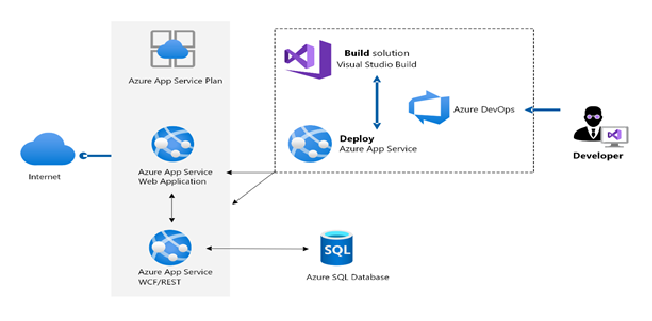
\includegraphics[width=0.8\textwidth]{img/architecture.png}
    \caption{Architecture logicielle 3-tiers de l'application}
    \label{fig:architecture}
\end{figure}
\vspace{0.5cm}

\section{Diagramme de déploiement}
L'architecture physique (infrastructure) définit la manière dont les différents composants logiciels sont déployés sur le réseau de l'entreprise.

\vspace{0.5cm}
\begin{figure}[H]
    \centering
    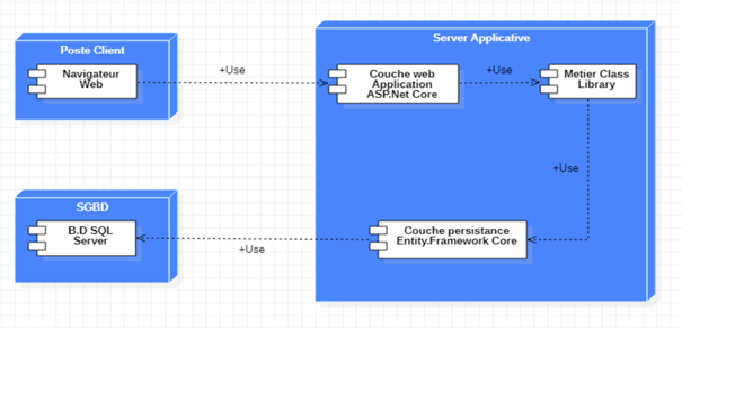
\includegraphics[width=0.9\textwidth]{img/Diagramme de déploiement.png}
    \caption{Diagramme de déploiement réseau de Cofat Capacity Study}
    \label{fig:deploiement}
\end{figure}
\vspace{0.5cm}

\textbf{Analyse de l'infrastructure réelle :} 
L'application est conçue pour fonctionner sur le réseau interne (Intranet) du Groupe COFAT pour des raisons évidentes de confidentialité.
\begin{itemize}
    \item \textbf{Poste Client} : Le Site Manager ou l'Acheteur utilise un navigateur web standard (Google Chrome ou Microsoft Edge). Le frontend React, servi initialement sur le port 4000 par le serveur web, s'exécute localement dans la mémoire du navigateur client.
    \item \textbf{Serveur d'Application (Node.js)} : Hébergé sur une machine virtuelle Linux chez ABM Informatique, l'API Express écoute les requêtes sur le port \textbf{9001}. Ce serveur possède également l'accès en écriture à deux répertoires de stockage : \texttt{/uploads/images} pour les photos des machines de référence, et \texttt{/uploads/budget} pour la sauvegarde temporaire des fichiers Excel importés avant leur traitement.
    \item \textbf{Serveur de Base de données (SQL Server)} : Hébergé sur un cluster sécurisé distinct de l'entreprise, écoutant sur le port TCP \textbf{1433}. Le serveur Express s'y connecte via des identifiants stockés dans des variables d'environnement (\texttt{.env}).
\end{itemize}

\section{Sprint 0 : Mise en place du socle technique}
Avant de coder la moindre interface utilisateur, la phase préparatoire du Sprint 0 s'est concentrée sur la création de la coquille vide de l'application et la configuration des dépendances npm essentielles.

\textbf{Côté Backend :}
Initialisation du projet Node via \texttt{npm init}, puis installation des briques logicielles essentielles :
\begin{verbatim}
npm install express sequelize mysql2 mssql tedious cors dotenv
            bcryptjs jsonwebtoken cookie-parser multer xlsx
\end{verbatim}
(Note : le paquet \textit{mssql} et son pilote sous-jacent \textit{tedious} sont requis pour la connexion à Microsoft SQL Server, tandis que \textit{mysql2} permet la compatibilité avec les bases MySQL/MariaDB, offrant une flexibilité de déploiement).\newline
L'arborescence serveur a été structurée de manière professionnelle :
\begin{itemize}
    \item \texttt{/models} : Les 11 fichiers Sequelize définissant le schéma de la BDD (\texttt{User.js}, \texttt{Site.js}, \texttt{Equipment.js}, \texttt{EquipmentPlanning.js}, \texttt{Spaces.js}, \texttt{HR.js}, \texttt{NonIndustrialBudget.js}, \texttt{BudgetNotification.js}, \texttt{Notification.js}, \texttt{StandardEquipment.js}, \texttt{StandardInvestment.js}).
    \item \texttt{/routers} : Les points d'entrée des requêtes HTTP, organisés par domaine métier (\texttt{nonIndustrialBudgetRoutes.js}, \texttt{standardInvestmentV2Routes.js}, \texttt{hrRoutes.js}, etc.).
    \item \texttt{/middlewares} : Scripts de vérification JWT (\texttt{authMiddlewares.js}) et d'autorisation de rôles (\texttt{compatibleAuth.js}).
    \item \texttt{/utils} : Utilitaires métier (\texttt{excelImporter.js} pour l'import/export Excel, \texttt{budgetNotificationHelper.js} pour le moteur de notifications).
\end{itemize}

\textbf{Côté Frontend :}
Génération du \textit{boilerplate} React via \texttt{npx create-react-app}. Installation des outils visuels, réseau et génération de fichiers :
\begin{verbatim}
npm install react-router-dom axios @mui/material antd recharts
            chart.js react-chartjs-2 lucide-react sweetalert2
            sweetalert2-react-content jspdf jspdf-autotable xlsx
            framer-motion i18next react-i18next
\end{verbatim}
L'arborescence client :
\begin{itemize}
    \item \texttt{/components} : Les blocs d'interface réutilisables, organisés par profil (\texttt{/admin}, \texttt{/user/pages}).
    \item \texttt{/Context} : Gestion globale de la session utilisateur (\texttt{AuthContext.js}).
    \item \texttt{/hooks} : Hooks métier personnalisés (\texttt{useNotifications.js}, \texttt{useTheme.js}, \texttt{useLanguage.js}).
    \item \texttt{/utils} : Utilitaires HTTP (\texttt{axiosInstance.js}, \texttt{authUtils.js}, \texttt{apiUtils.js}).
    \item \texttt{/services} : Services de notifications (\texttt{NotificationService.js}).
\end{itemize}

\section{Sprint 1 : Authentification et Administration Globale}
L'objectif du premier vrai sprint de développement était de verrouiller l'application et de fournir les outils d'administration à la Direction de COFAT. 

\subsection{Processus d'authentification sécurisée}
La page de Login (Figure \ref{fig:login}) est la porte d'entrée unique. 

\vspace{0.5cm}
\begin{figure}[H]
    \centering
    
\includegraphics[width=0.7\textwidth]{img/LOGIN.png}
    \caption{Interface d'authentification de l'application}
    \label{fig:login}
\end{figure}
\vspace{0.5cm}

\textbf{Description du diagramme de séquence d'authentification (Figure \ref{fig:seq_auth}) :}
Lorsqu'un utilisateur saisit ses identifiants, le scénario technique, tel qu'illustré dans le diagramme de séquence UML du rapport, se déroule en plusieurs étapes strictes :
1. Le client React envoie une requête \texttt{POST /api/auth/login} contenant l'email et le mot de passe en clair.
2. Le routeur Express passe la main au contrôleur d'authentification.
3. Sequelize exécute un \texttt{findOne} sur la table \texttt{Users} pour vérifier l'existence de l'email.
4. Si l'utilisateur existe, la bibliothèque \texttt{bcrypt} exécute la fonction \texttt{bcrypt.compare()} pour comparer le hash stocké en BDD avec le mot de passe fourni.
5. Si la comparaison est un succès, Node.js génère un jeton d'accès via \texttt{jwt.sign()}, y incluant l'ID, le site et le Rôle de l'utilisateur (ex: Admin).
6. Le jeton est renvoyé au navigateur via la fonction \texttt{res.cookie('token', token, \{ httpOnly: true \})}.
7. Le frontend détecte le succès, met à jour l'état \textit{AuthContext}, et le module \textit{React Router} effectue une redirection vers le menu principal adapté au profil.

\vspace{0.5cm}
\begin{figure}[H]
    \centering
    
\includegraphics[width=0.8\textwidth]{img/DiagrammeSeqAuthentification.png}
    \caption{Diagramme de séquence du processus d'authentification JWT}
    \label{fig:seq_auth}
\end{figure}
\vspace{0.5cm}

\subsection{Le Tableau de Bord Administrateur (Admin Dashboard)}
Une fois authentifié en tant qu'Admin, l'utilisateur atterrit sur son espace dédié (Figure \ref{fig:dashboard_admin} et \ref{fig:home_page}). 

\vspace{0.5cm}
\begin{figure}[H]
    \centering
    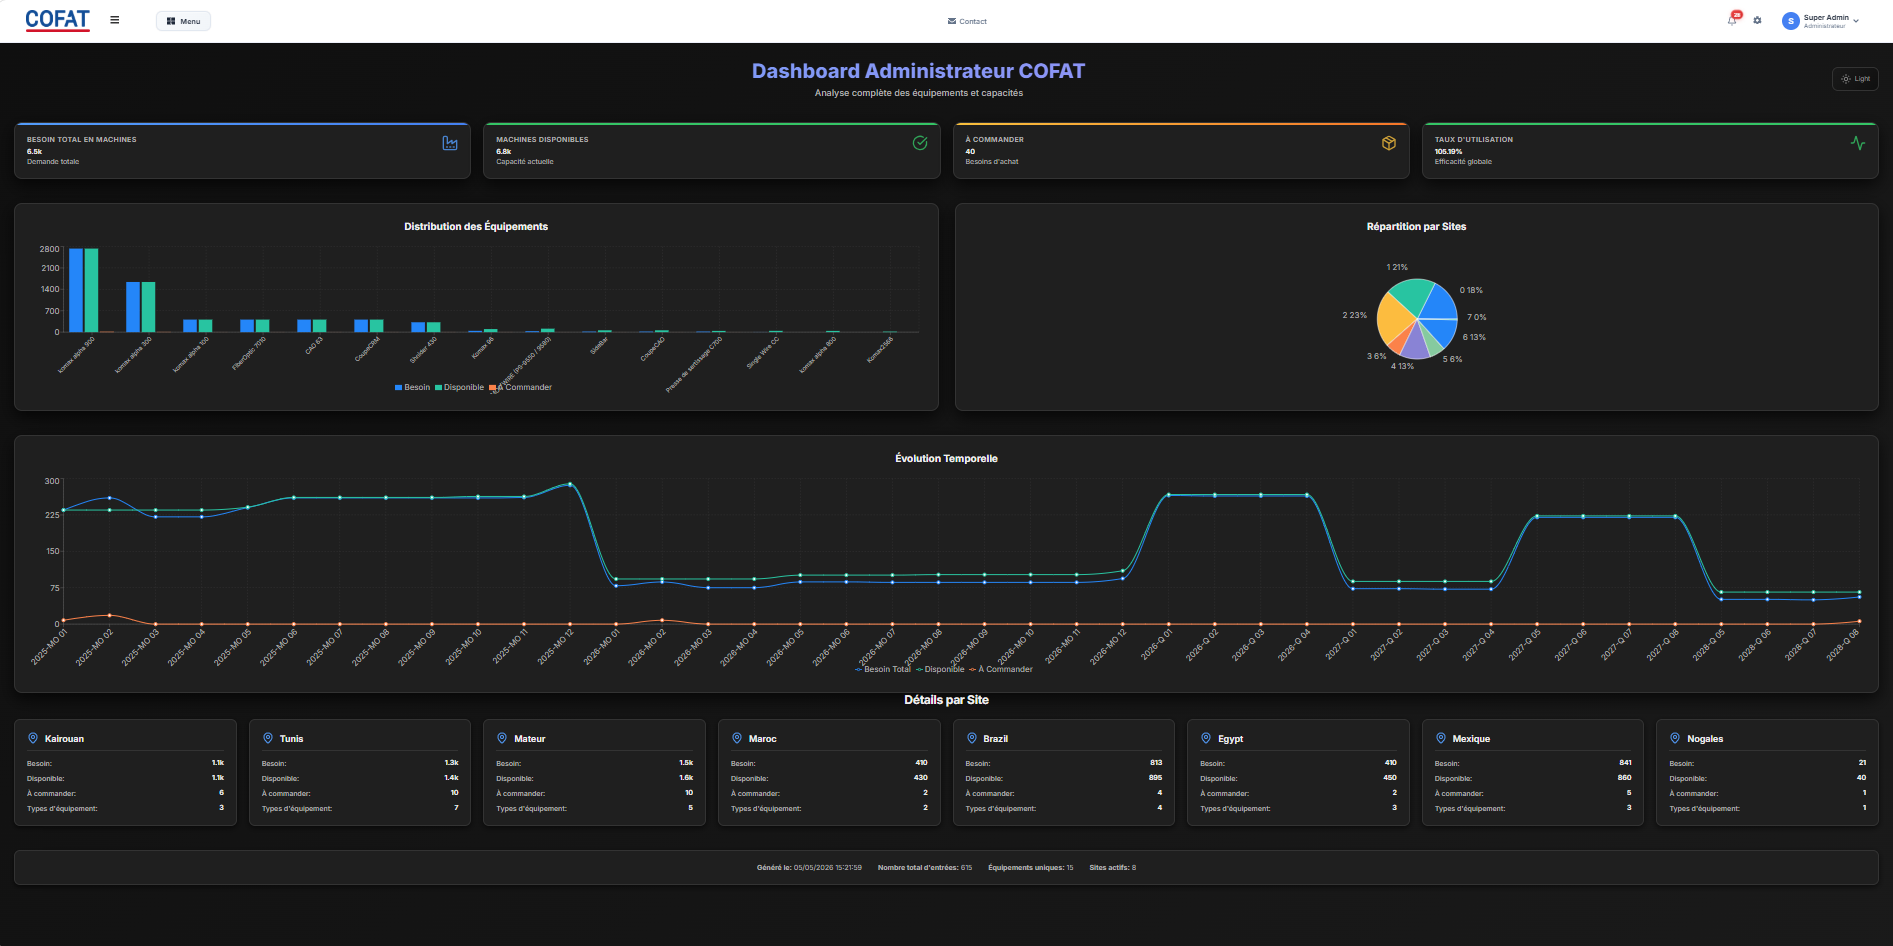
\includegraphics[width=0.8\textwidth]{img/dashboard admin.png}
    \caption{Tableau de bord de l'Administrateur}
    \label{fig:dashboard_admin}
\end{figure}
\vspace{0.5cm}

\vspace{0.5cm}
\begin{figure}[H]
    \centering
    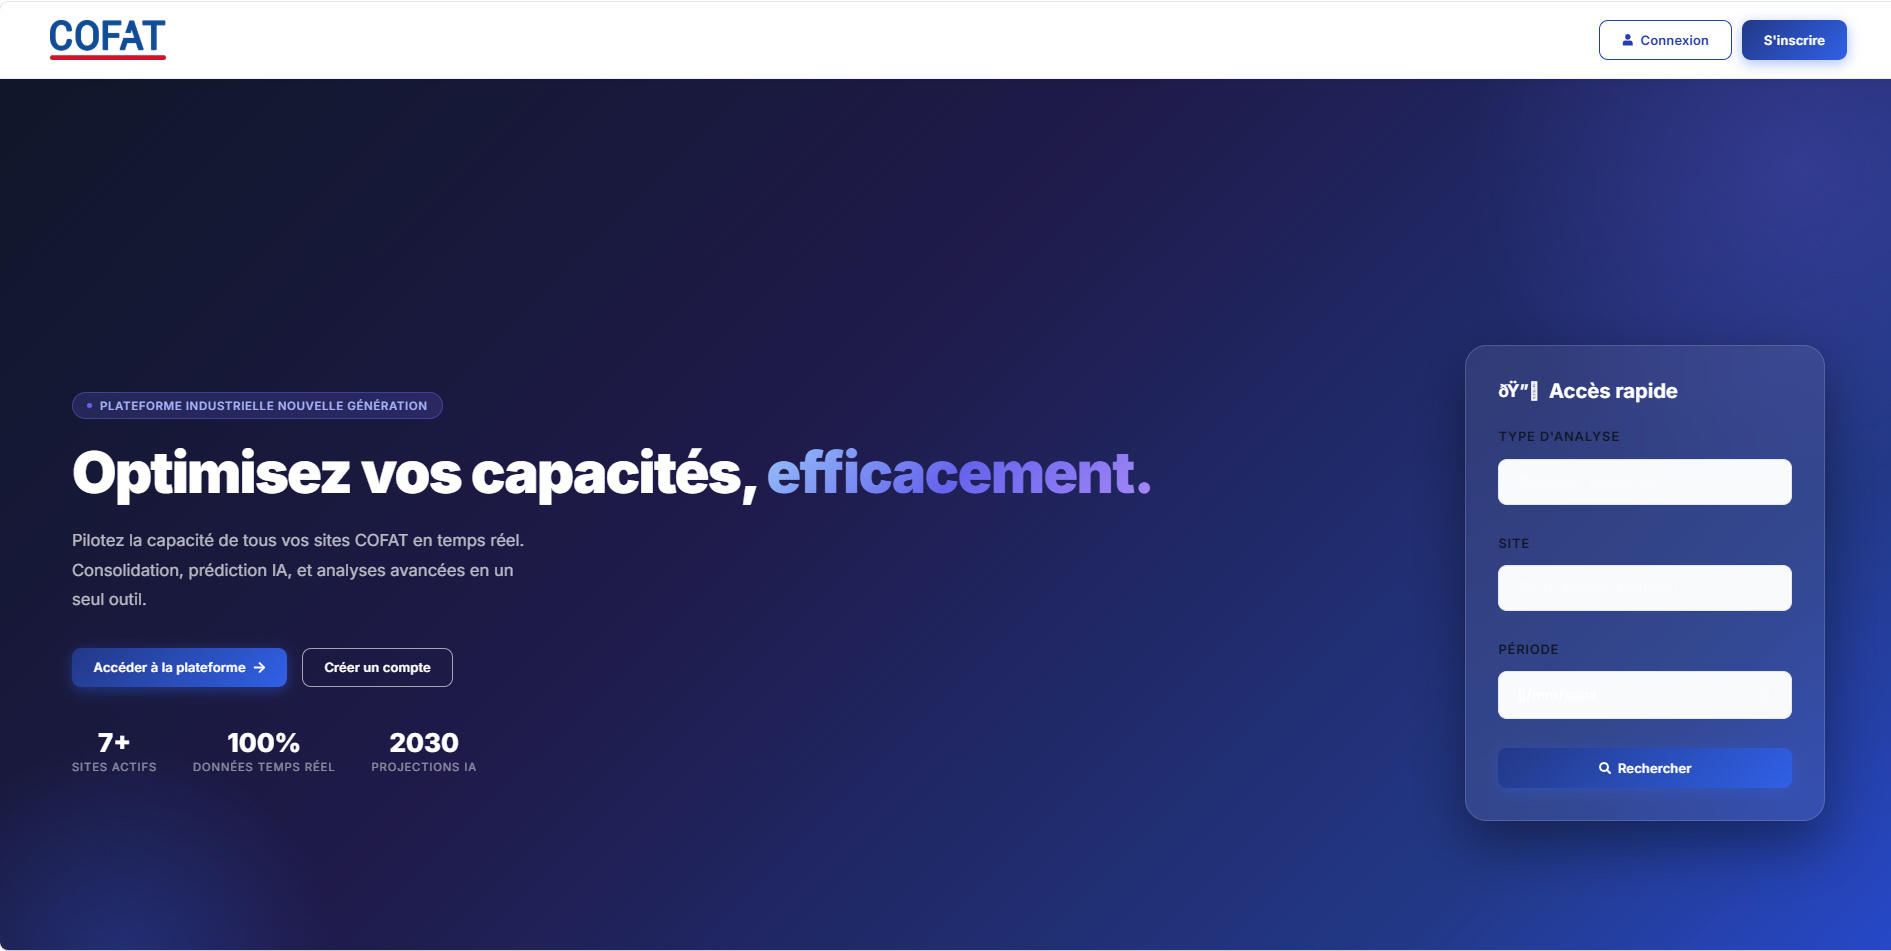
\includegraphics[width=0.8\textwidth]{img/HOME PAGE.png}
    \caption{Menu de navigation principal (Home Page)}
    \label{fig:home_page}
\end{figure}
\vspace{0.5cm}

\textbf{Description des fonctionnalités de l'interface :}
Le Dashboard est structuré de manière ergonomique avec une barre de navigation latérale (Sidebar) persistante. Depuis cet espace, l'Administrateur a accès aux modules vitaux du système :
\begin{itemize}
    \item \textbf{Gestion des Utilisateurs} : Un tableau CRUD permettant de créer des comptes pour les nouveaux ingénieurs, de leur assigner un mot de passe temporaire et de définir leur périmètre (Site de rattachement) et leur rôle strict (Admin, Site Manager, Achat).
    \item \textbf{Gestion des Sites} : Ajout de nouvelles entités industrielles (Code du site, pays, type) qui alimenteront dynamiquement les menus déroulants de toute l'application.
    \item \textbf{Accès aux Consolidations (Cofat Group)} : Raccourcis directs vers les vues mondiales des équipements et ressources humaines, affichant des tuiles de synthèse (KPIs) globales en haut de l'écran.
    \item \textbf{Catalogue StandardInvestment} : Accès centralisé au référentiel d'investissement du groupe.
\end{itemize}
La navigation est extrêmement fluide car il s'agit d'une SPA (Single Page Application) ; les composants React se montent et se démontent instantanément sans rafraîchissement global de la page web.

\section{Conclusion}
Au cours de ce chapitre, nous avons justifié et matérialisé l'architecture logicielle de \textit{Cofat Capacity Study}. Les choix de Node.js, Express, React et MS SQL Server apportent une robustesse et une évolutivité à la hauteur des enjeux de l'industrie automobile. La mise en place de l'architecture 3-tiers et le succès du Sprint 1 (déploiement du socle technique, sécurisation par JWT et interface d'administration) prouvent la viabilité technique de notre approche. 
Le socle étant désormais solidement en place, le chapitre 4 explorera en profondeur le cœur métier de la plateforme : le développement des interfaces de "Planification Locale" pour les usines (Sprint 2) et la prouesse algorithmique de la "Consolidation Groupe" en temps réel (Sprint 3).